\part{Praktická část}

\chapter{Cíl projektu}

V praktické části mé práce jsem vytvořil vlastní hru pro VR. Stanovil jsem si následující kritéria:

\begin{itemize}
  \item \textbf{Nenáročnost}. Chtěl jsem, aby má hra nebyla obtížná na pochopení. Většina VR her vyžaduje zvýšenou fyzickou aktivitu nebo hlubší porozumění VR konceptů. Ideálně jsem chtěl vytvořit hru, kterou bych mohl komukoliv půjčit, aniž bych musel dlouze vysvětlovat její princip.
  \item \textbf{Grafická jednoduchost}. Nepovažuji se za umělce a umím vytvářet pouze základní modely a textury. Bylo pro mě tedy klíčové přijít s takovým konceptem, který by byl vzhledově nenáročný.
  \item \textbf{Interaktivita}. Od své hry jsem chtěl, aby doopravdy využívala funkce, které VR platformy poskytují. Tedy ovládání pohybem, jednoduchá fyzika atp.
\end{itemize}

Dospěl jsem k následujícímu návrhu: Hra sestává z kostky tvořené úrovněmi naskládanými na sebe. Každá úroveň představuje bludiště, skrze které musí nakláněním hráč navigovat kuličku. Při dosažení cíle je úroveň odebrána, kostka se zmenší a je odhalena další úroveň.

To splňuje moje kritéria - hra je jednoduchá, na vykreslení potřebuje jen geometrické tvary a vyžaduje pohyb rukama pro naklánění bludiště.

Již od samého začátku jsem svou hru chtěl napsat v herním enginu. Herních enginů zdarma, které zároveň podporují XR, není mnoho. Zvolil jsem si svobodný Godot Engine.

\chapter{Herní engine Godot}

Godot je bezplatný herní engine. Hlavní důvod, proč jsem si jej vybral namísto známějšího Unity, je jeho licence. Godot je šířen pod svobodnou licencí MIT, která vývojářům dovoluje kód používat komerčně i naopak, a to pod jedinou podmínkou: text licence je ve výsledné práci zachován. Unity Engine je naopak distribuován pod nesvobodnou licencí a za některé funkce musí vývojáři platit. Godot se v poslední době stává více a více populárním a obdržel investice od velkých společností. Mezi ně patří např. grant od Epic Games pro vývoj grafiky a grant od Mety pro vývoj XR funkcí. \cite{godot_epicgames} \cite{godot_meta}

Pro úpravu Godot projektů používáme oficiální editor. Základními stavebními bloky enginu jsou uzly, které jsou uspořádány do stromu, podobně jako jsou webové stránky reprezentovány stromem značek. Tyto uzly samy o sobě nemají mnoho funkcí, jejich kombinací ale můžeme dosáhnout komplexnějšího chování. Jednotlivé uzly se dají přirovnat k třídám v objektově orientovaném programování, které se navzájem rozšiřují.

Například uzel \texttt{Node3D} disponuje atributem \texttt{position} (pozice) a uzel \texttt{Camera3D}, který rozšiřuje \texttt{Node3D}, disponuje atributy \texttt{position} a \texttt{fov} (field of view; zorný úhel). Dceřinné uzly zároveň dědí atributy rodičovských uzlů, pokud oba rozšiřují společný uzel (pokud je např. \texttt{Camera3D} dceřinný uzel \texttt{Node3D}, pak se \texttt{Camera3D} pohybuje společně s \texttt{Node3D} (sdílí atribut \texttt{position}) a \texttt{position} na \texttt{Camera3D} je relativní posun od \texttt{Node3D})

Uzlům můžeme přiřadit \textit{skript}, který upravuje jejich chování. Tento skript se chová jako třída v OOP, která rozšiřuje daný uzel. Pokud rozšiřujeme uzel pro 2D grafiku, můžeme metodou získat pozici jako 2D vektor. Pokud rozšiřujeme uzel pro 3D grafiku, stejnou metodou můžeme získat pozici jako 3D vektor. Stejně tak můžeme přepisovat virtuální funkce. Projekty v Godotu používají dedikovaný jazyk zvaný GDScript, existuje ale oficiální podpora jazyka C\# a komunitně vytvořená rozšíření pro Rust.

Uzel a jeho dceřinné uzly společně s přiřazenými skripty můžeme dále uložit jako izolovanou \textit{scénu} (textový soubor .tscn), kterou můžeme poté instancovat. Scéna se pak chová jako samostatný uzel. Jedna scéna je vždy hlavní scénou a je otevřena při spuštění projektu.

\begin{figure}[H]
  \centering
  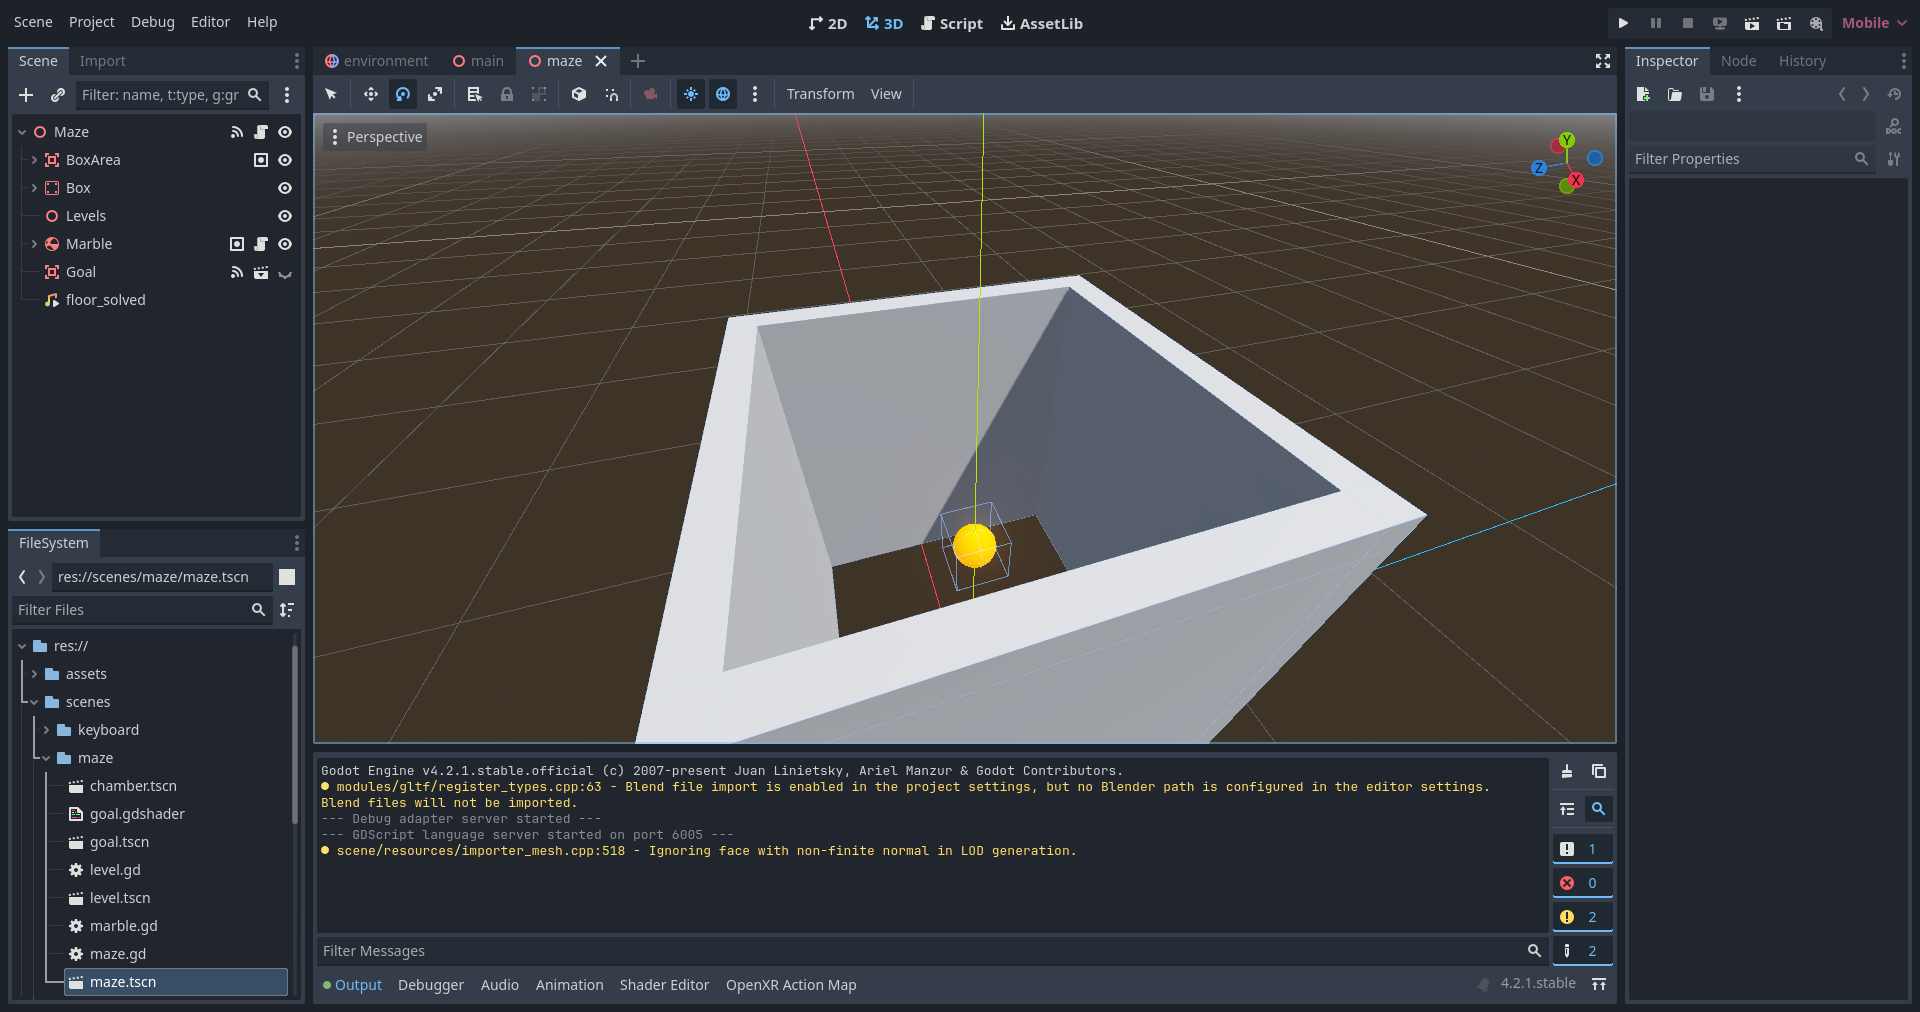
\includegraphics[height=180pt]{godot_editor.png}
  \caption{Editor Godot Engine a otevřená scéna Maze.tscn}
  \label{godot_editor_maze_tscn}
\end{figure}

\section{Jazyk \textit{GDScript}}

GDScript je jazyk, ve kterém se vyvíjí většina Godot projektů. Můj projekt je taktéž psán v GDScriptu a z tohoto důvodu jej zde popisuji pro snadnější pochopení kódu.

GDScript je vysokoúrovňový, objektově orientovaný, imperativní a hybridně (staticky i dynamicky) typovaný jazyk. Vzhledově nápadně připomíná jazyk Python a podobně jako Python používá indentaci pro vyjádření řídící struktury. Nabízí širokou škálu vestavěných tříd pro manipulaci s hodnotami typickými pro hry, matematiku a fyziku (textury, vektory, matice) a obecné typy (celé číslo, desetinné číslo, textový řetězec atd.). Proměnné programátor může anotovat typem. Podporuje koprogramy (coroutines) a událostmi řízené programování pomocí "signálů". Pro svou hlubokou integraci se samotným enginem je vhodný pro jednoduché projekty, kvůli své dynamičnosti ovšem nenabízí stejnou rychlost jako kompilované jazyky. \cite{gdscript_reference}

Níže je příklad kódu v GDScriptu.

\lstinputlisting{code/sample_gdscript.gd}

\chapter{Struktura projektu}

\begin{samepage}
  Můj projekt jsem rozdělil do jednotlivých, jednoduše spravovatelných scén. Tímto jsem mohl na mnohých funkcích pracovat odděleně a mohl bych je, teoreticky, použít i v budoucích projektech. Zde je zjednodušený diagram těchto scén:

  \vspace{0.3cm}
  \renewcommand\DTstyle{\rmfamily}
  \dirtree{%
    .1 Hlavní scéna (spojuje a ovládá zbylé scény) .
    .2 Prostředí (skybox) .
    .2 Hráč .
    .3 Trackované ovladače, kamera synchronizovaná s headsetem .
    .2 Obrazovka .
    .3 Výběr obtížnosti, žebříček nejlepších, nastavení hry .
    .2 Kostka s bludištěm .
    .3 Kostka o určité velikosti .
    .4 Úroveň (bludiště, ze kterých se kostka skládá) .
    .5 Komnata (buňky, ze kterých se skládá bludiště) .
    .3 Kulička (volně se pohybující předmět s vlastní fyzikou) .
  }

  Každá scéna reprezentuje odlišnou sadu problémů a výzev, které jsem musel při tvorbě projektu řešit.
\end{samepage}

\section{Hráč, interakce se zařízením}

Scéna s hráčem je přímo spojena s headsetem a sledovanými ovladači. Sestává z uzlů \texttt{XRCamera3D}, pohledu do 3D prostředí synchronizovaným s umístěním headsetu, a dvou uzlů \texttt{XRController3D}, které jsou synchronizované s umístěním levého a pravého ovladače.

K tomuto jsem použil svobodnou knihovnu Godot XR Tools, která nabízí podpůrné scény pro XR projekty. Z té jsem si zapůjčil kód nutný k inicializaci VR headsetu a 3D model ruky licencovaný pod CC0\footnote{CC0 je licence používána pro díla ve veřejné doméně. Autoři modelu se vzdali autorských práv.}.

Kvůli prevenci závratí jsem do této scény přidal platformu umístěnou pod hráčem ve výšce, kterou si ve svém zařízení předem nastavil jako výšku podlahy. Hráč poté nemá pocit, že se "vznáší v prázdnotě".

Účel scény je kromě správného zobrazení hry také interpretace vstupu od hráče. Ve hře jsou klíčové dvě funkce: uchopení nějakého předmětu (např. kostky pro její naklánění) a interakce s uživatelským rozhraním pomocí laserového ukazovátka. Druhý zmíněný bod popisuji podrobněji v sekci \ref{uzivatelske_rozhrani}.

Implementovat uchopení předmětu \textit{jednou rukou} je triviální -- Stačí, aby tento objekt sledoval změny v transformaci uzlu \texttt{XRController3D}. Uchopení \textit{oběma rukama}, chování, kterého jsem chtěl dosáhnout ve své hře, je ale složitější. Protože je možné ovladače volně pohybovat a neexistují žádná fyzická omezení (hráč by mohl předmět např. volně kroutit), musel jsem přistoupit ke kompromisu. Při sevření obou ovladačů hra vytvoří neviditelný uzel, jehož změny v transformaci uchopený předmět sleduje. Tento uzel je manuálně umístěn do středu mezi levým a pravým ovladačem (=průměru jejich pozic; pokud je považujeme za vektory) a je otočen tak, že vektor Z tranformační matice\footnote{Godot Engine používá pro rotaci uzlů transformační matice. Vektor Y míří vzhůru.} míří od levého ovladače k pravému ovladači a vektor Y míří stejným směrem jako palce uživatele. Tímto jsem dosáhl poněkud přesvědčivého efektu.

TODO: Přidat foto s ilustrací co to dovysvětlí.

\section{Kostka, bludiště}

Kostka (a bludiště v ní) je hlavním prvkem hry. Skládá se ze čtyř zdí, úrovní (bludišť) a komnat. Každé bludiště je v podstatě mřížka čtvercových buněk, které jsou odděleny zdmi. Jedna buňka je označena jako začátek a jedna jako cíl.

\begin{figure}[H]
  \centering
  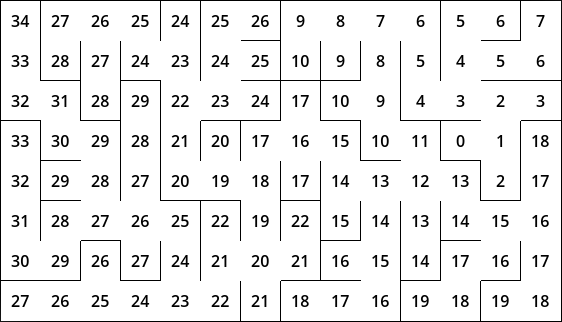
\includegraphics[height=180pt]{maze_example.png}
  \caption{Ukázka vygenerovaného bludiště (v 2D podobě) z testovací scény}
  \label{maze_example}
\end{figure}

Pro vygenerování bludiště jsem použil Wilsonův algoritmus. Důvodem je fakt, že tento algoritmus nemá sklony vytvářet extrémně dlouhé či extrémně krátké chodby, narozdíl od jiných algoritmů pro generování bludiště. Postup je následující: \cite{enwiki:1193338583}

\begin{enumerate}
  \setcounter{enumi}{0}
  \item Mějme graf buněk, kde má každá buňka několik sousedních buněk (např. pro mřížku mají buňky 4 sousední buňky, vyjma těch na krajích a v rozích). Nechť je mezi všemi sousedícími buňkami spojení, které lze označit jako průchod nebo zeď.
  \item Označme všechny spojení jako zdi a jednu náhodně zvolenou buňku označme jako zahrnutou v bludišti.
  \item Libovolným způsobem zvolme buňku. Pokud je tato buňka zahrnuta v bludišti, zvolme jinou buňku. \label{pick}
  \item Označme buňku jako zahrnutou v současné iteraci.
  \item Přejděme na náhodnou sousedící buňku a v předchozí buňce uložíme ukazatel k následující buňce. Poté: \label{lerw}
        \begin{itemize}
          \item Pokud tato buňka není zahrnuta ani v iteraci, ani v bludišti, označme ji jako zahrnutou v iteraci a přejděme na krok \ref{lerw}.
          \item Pokud je tato buňka zahrnuta v iteraci, vznikla smyčka. Pomocí ukazatelů uložených v buňkách projděme tuto smyčku, odstraňme buňky ze současné iterace a odeberme ukazatele.
          \item Pokud je tato buňka zahrnuta v bludišti, všechny buňky v iteraci označme jako buňky v bludišti. Spoje mezi buňkami v této iteraci označme jako průchody.
        \end{itemize}
  \item Pokud stále existují buňky, které nejsou zahrnuty v bludišti, přejděme zpět ke kroku \ref{pick}.
\end{enumerate}

\begin{figure}[H]
  \centering

  \begin{minipage}{.5\textwidth}
    \centering
    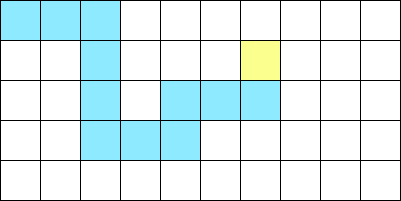
\includegraphics[height=100pt]{maze_gen_step_1.png}
  \end{minipage}%
  \begin{minipage}{.5\textwidth}
    \centering
    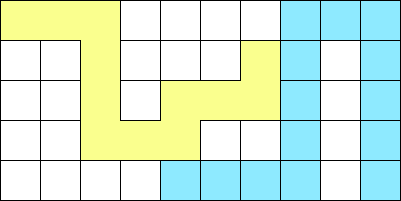
\includegraphics[height=100pt]{maze_gen_step_2.png}
  \end{minipage}

  \caption{Příklad dvou iterací kroků \ref{pick} až \ref{lerw}. Žlutě jsou buňky v bludišti, modře buňky v iteraci.}
\end{figure}

\begin{figure}[H]
  \centering
  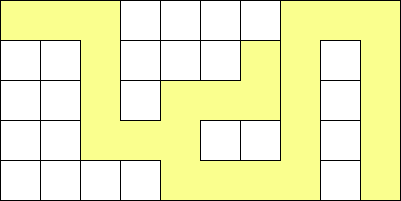
\includegraphics[height=120pt]{maze_gen_step_3.png}
  \caption{Stav po těchto dvou iteracích}
\end{figure}

todo:
- sestavení vygenerovaného bludiště v godot enginu
- kód algoritmu v GDScriptu
- následná úprava pro určení nejvzdálenějšího bodu

\label{uzivatelske_rozhrani}
\section{Uživatelské rozhraní}

todo:
- Obrazovky
- použití raycastu pro zjištění kolize s laserovým ukazovátkem